\documentclass[../main.tex]{subfiles}
\graphicspath{{\subfix{../images/}}}

\begin{document}

\section{7-Segment Display Driver}

\subsection{LedDecoder module}

Στόχος αυτού του module ήταν να δέχεται ως είσοδο ένα σύμβολο 4 bits και να
βγάζει ως έξοδο 6 bits με τα οποία θα ελέγχεται μια οθόνη 7 τμημάτων (με το
7\textsuperscript{ο} bit \textit{DP} να είναι πάντα 1). 

\subsubsection*{Υλοποίηση}

Η υλοποίηση ήταν πολύ απλή με την χρήση ενός always block για την δημιουργία
μιας ασύγχρονης read-only μνήμης. Αυτό φαίνεται και στο
Σχήμα~\ref{fig:module_led_decoder} που έκανε σύνθεση το εργαλείο yosys.

\begin{figure}[H]
  \begin{center}
    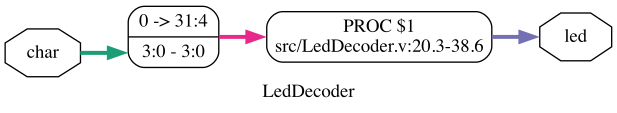
\includegraphics[width=0.5\textwidth]{../../diagrams/LedDecoder.png}
  \end{center}
  \caption{Σύνθεση του LedDecoder με yosys.}
  \label{fig:module_led_decoder}
\end{figure}

\subsubsection*{Επαλήθευση}
Για την επαλήθευση της σωστής λειτουργίας δημιουργήθηκε ένα testbench που
δίνονται οι τιμές από 0 έως 13 ως char και λαμβάνουμε τις αναμενόμενες τιμές
για τα 6 bits των led.

\begin{figure}[H]
  \begin{center}
    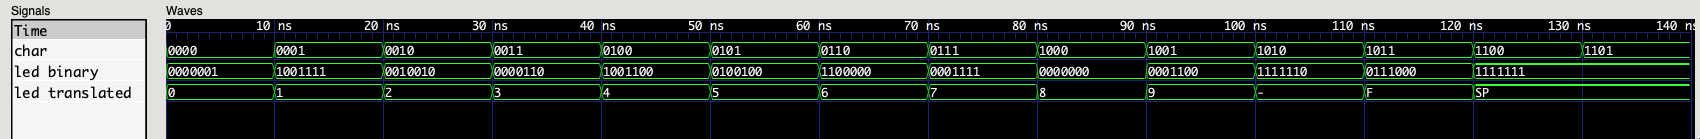
\includegraphics[width=\textwidth]{../images/led_decoder_tb.png}
  \end{center}
  \caption{LedDecoder testbench}
  \label{fig:tb_led_decoder}
\end{figure}

\subsection{LedDriver4 module}

Στόχος αυτού το module ήταν να οδηγεί 4 οθόνες 7 τμημάτων με την χρήση ενός
\textit{LedDecoder}. Δηλαδή θα πρέπει να δέχεται ένα μήνυμα τεσσάρων συμβόλων
άρα 16 bits και με τους κατάλληλους χρονισμούς να δείχνει τα πρώτα 4 bit στην
πρώτη οθόνη, τα επόμενα 4 στην δεύτερη κτλ.. Έχοντας λοιπόν ως εξόδους 4 bits
για τις ανόδους της κάθε οθόνης και 6 bits τα οποία θα είναι κοινά και θα
οδηγούν τα led των οθονών, μπορούμε να φορτώνουμε το σύμβολο που θέλουμε να
εμφανιστεί και μετά να οδηγούμε στην άνοδο της οθόνης που θέλουμε να ανάψουμε
στο 0. Κάνοντας την παραπάνω διαδικασία κυκλικά με μεγάλη συχνότητα θα φαίνεται
ότι όλες οι οθόνες είναι αναμμένες.

\subsubsection*{Υλοποίηση}

Η υλοποίηση έγινε με την χρήση ενός FSM με 16 καταστάσεις που φαίνεται στο
Σχήμα~\ref{fig:fsm_led_driver}, πηγαίνοντας στην επόμενη κατάσταση κάθε 16
κύκλους του 50MHz ρολογιού. Στο Σχήμα~\ref{fig:module_led_driver} φαίνεται η
σύνθεση του εργαλείου yosys για αυτό το module, το οποίο εμπεριέχει και το
\textit{LedDecoder} module.

\begin{figure}[H]
  \begin{center}
    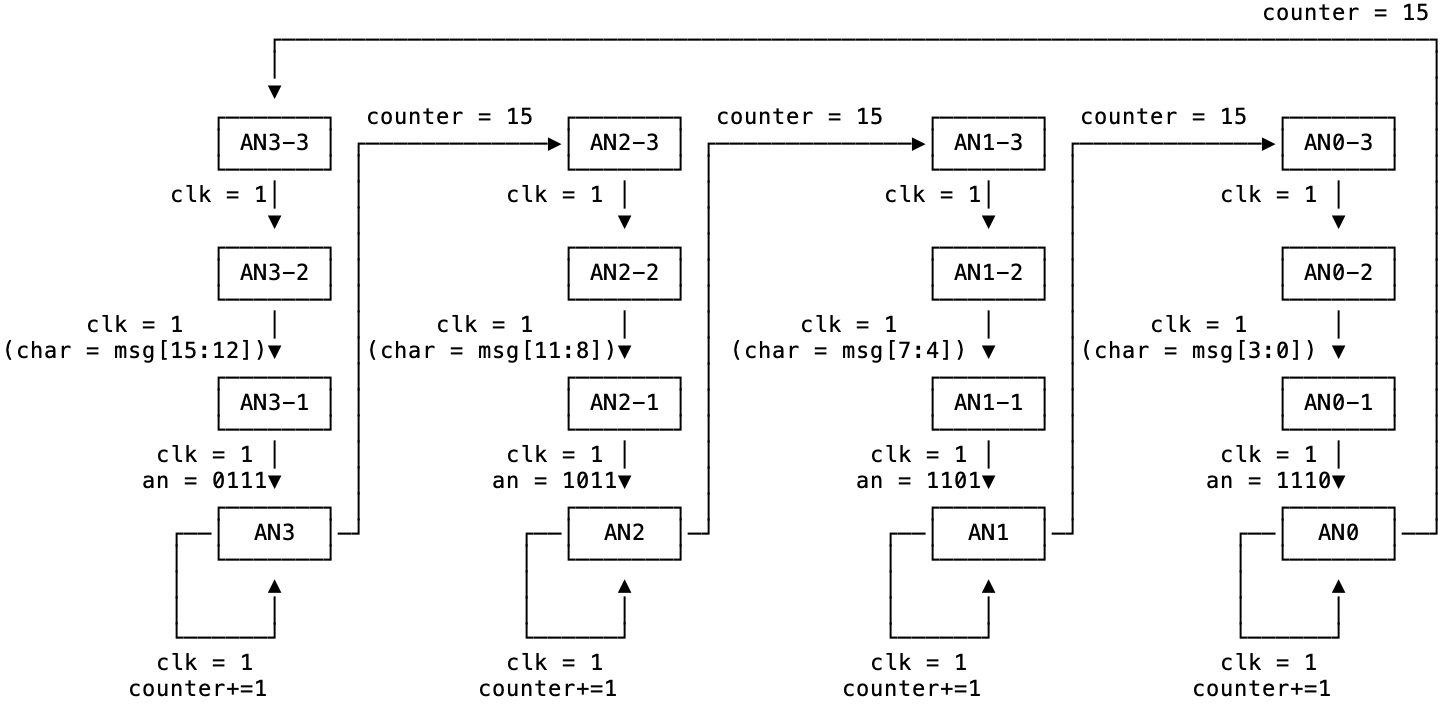
\includegraphics[width=0.7\textwidth]{../../monodraw/LedDriver4.png}
  \end{center}
  \caption{FSM του LedDriver4.}
  \label{fig:fsm_led_driver}
\end{figure}

\begin{figure}[H]
  \begin{center}
    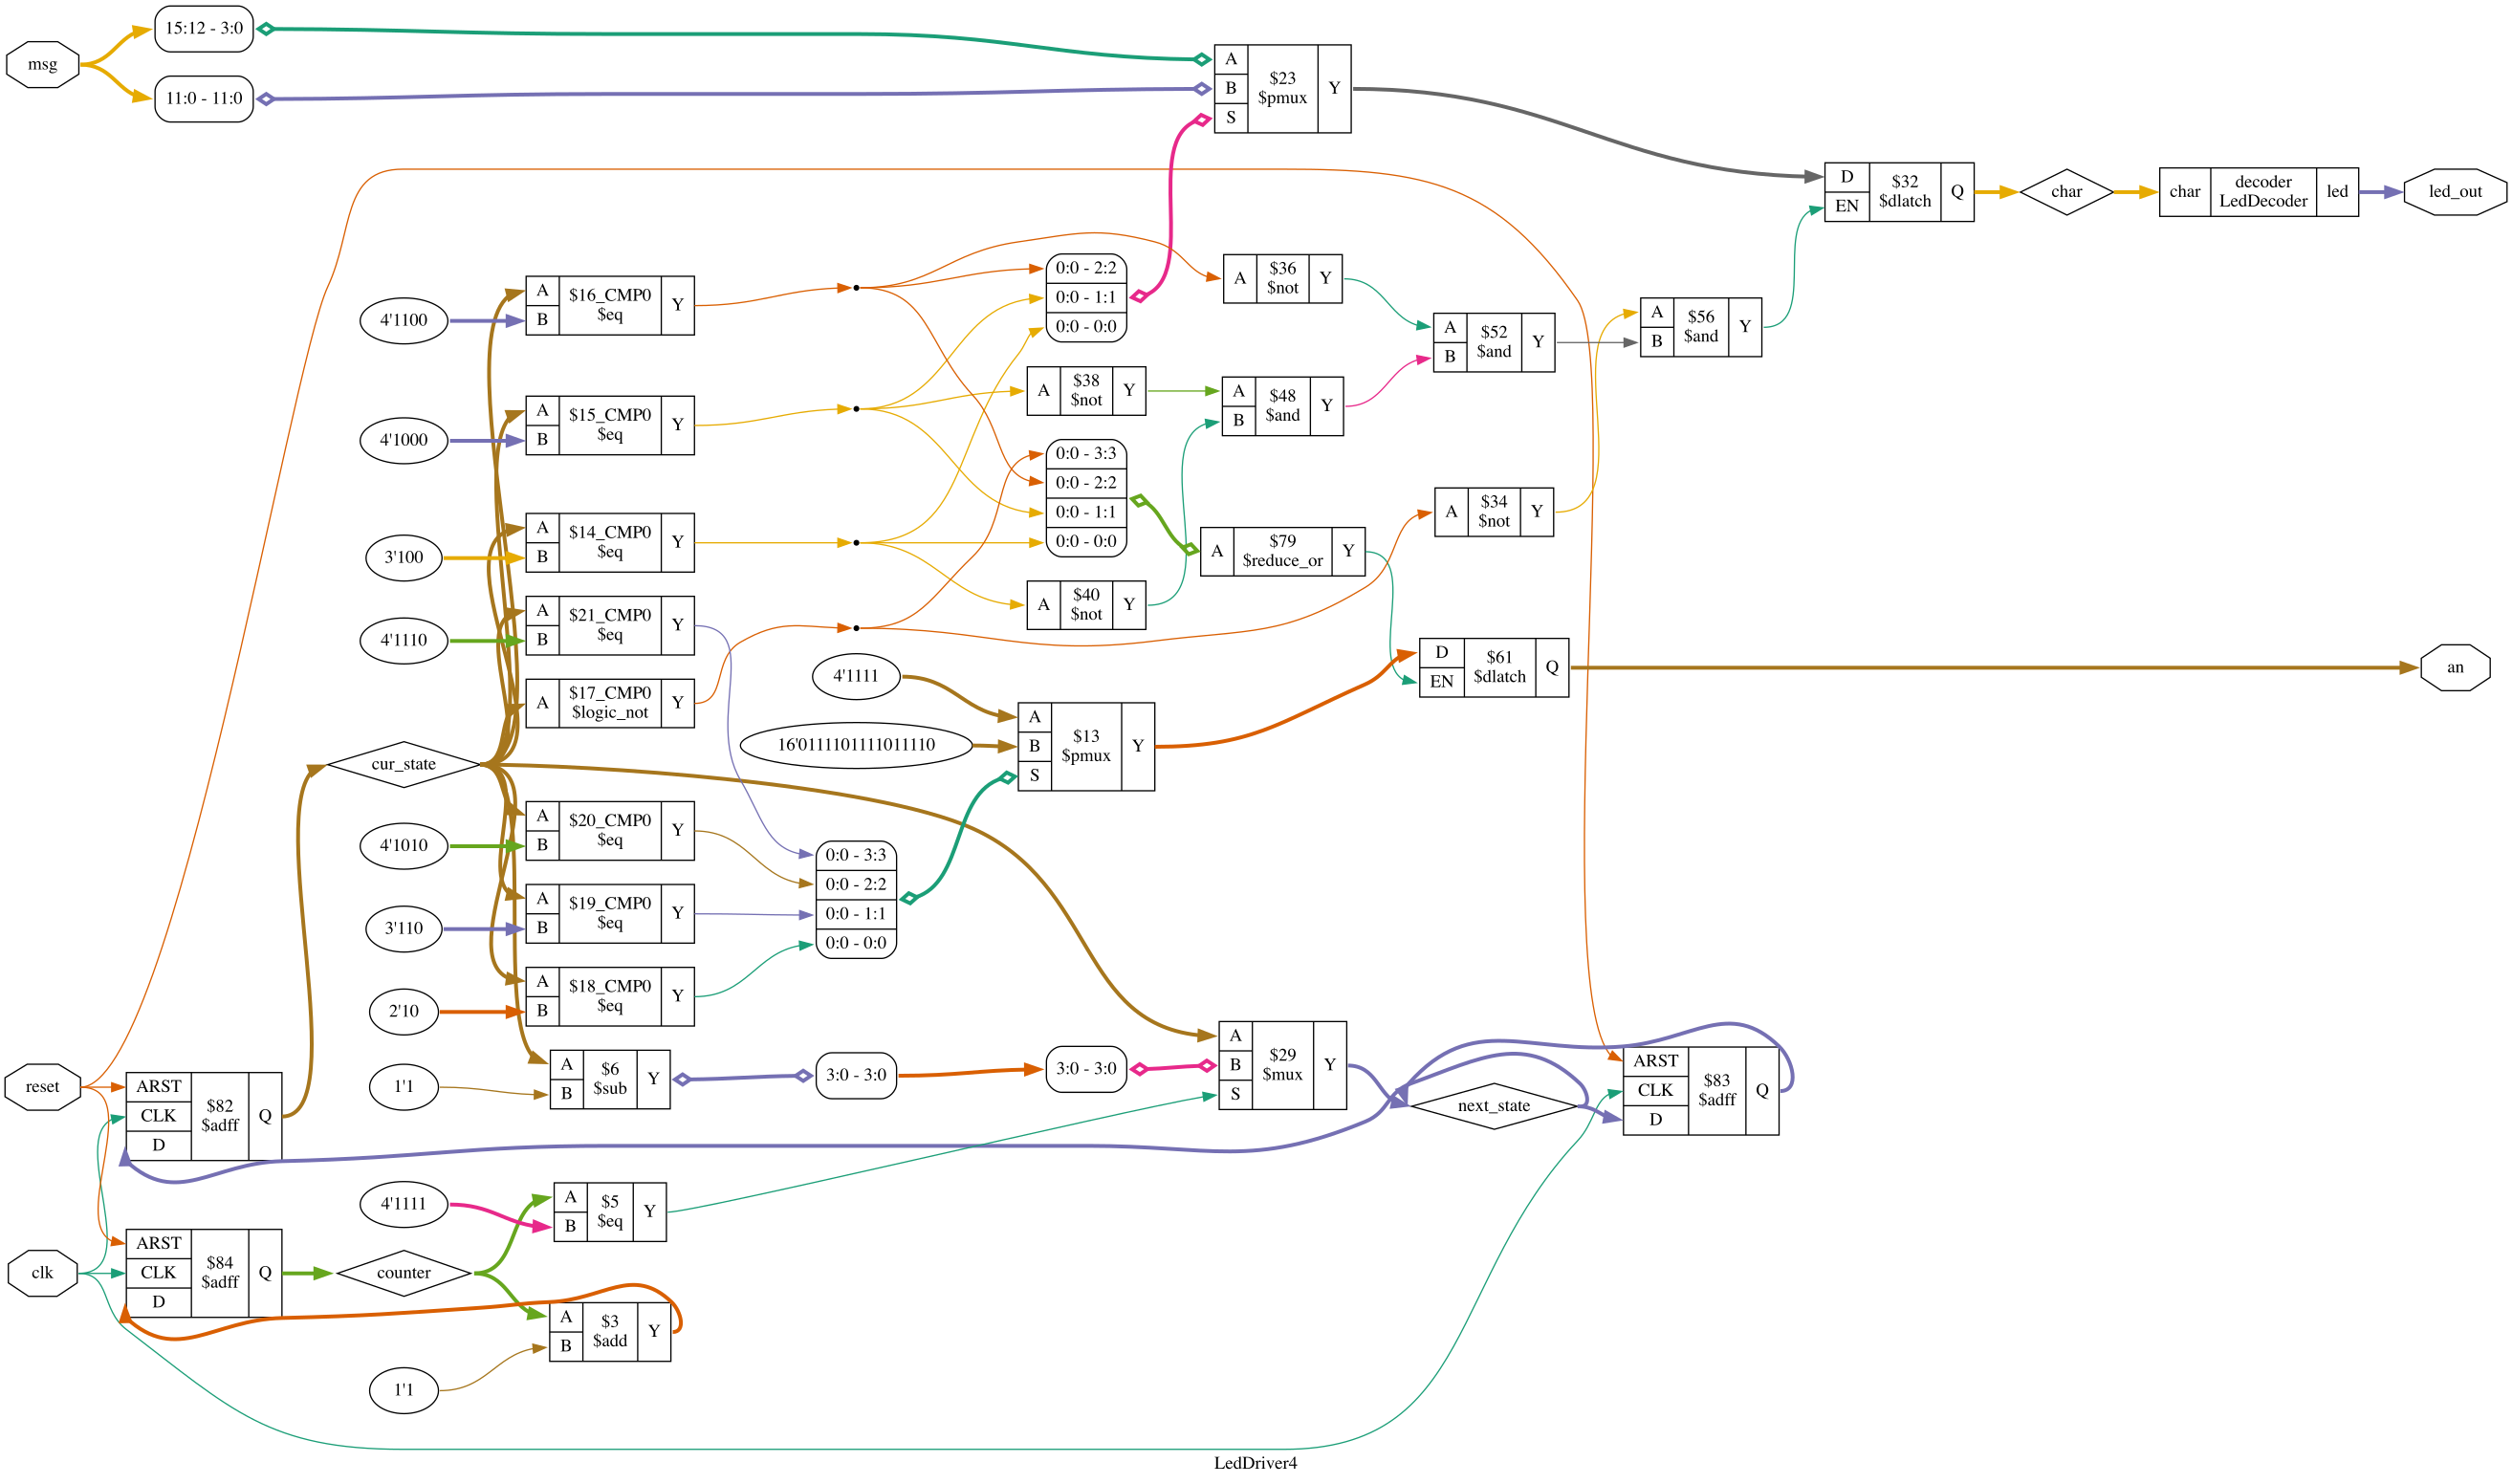
\includegraphics[width=\textwidth]{../../diagrams/LedDriver4.png}
  \end{center}
  \caption{Σύνθεση του LedDriver4 με yosys.}
  \label{fig:module_led_driver}
\end{figure}

\subsubsection*{Επαλήθευση}

Για την επαλήθευση της σωστής λειτουργίας δημιουργήθηκε ένα testbench που
δίνονται ως είσοδοι τα μηνύματα "-194", "  10", "- 32" και "FFFF". Στο
Σχήμα~\ref{fig:tb_led_driver_zoomed_out} φαίνεται πως τα μηνύματα μεταφράζονται
σωστά ανά 4 bits και πως κάθε άνοδος άγει για κάποιο χρονικό διάστημα.

Μεγεθύνοντας στην διάρκεια μεταδόσεις ενός μηνύματος
(Σχήμα~\ref{fig:tb_led_driver}) μπορούμε να μετρήσουμε την διάρκεια που άγει η
κάθε άνοδος, δηλαδή την διάρκεια από το marker A έως B. Η διάρκεια αυτή είναι
320ns όπως ήταν αναμενόμενο αφού θέλαμε να άγει για 16 κύκλους του ρολογιού
$16\times20=320ns$. Επίσης η διάρκεια που δεν άγει καμία άνοδος είναι σωστά
$3\times320=960ns$ (από B έως C marker).

\begin{figure}[H]
  \begin{center}
    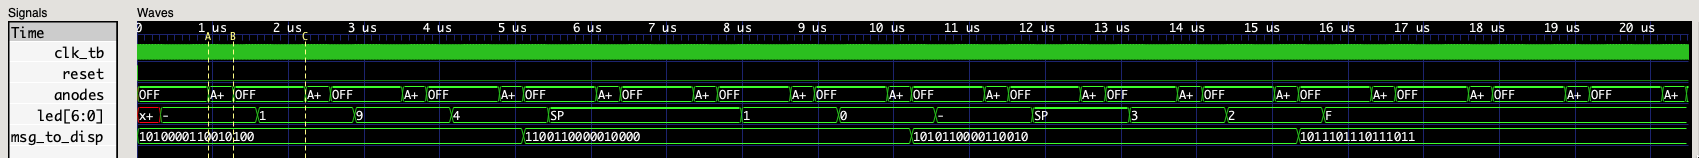
\includegraphics[width=\textwidth]{../images/led_driver_tb_zoomed_out.png}
  \end{center}
  \caption{LedDriver4 testbench.}
  \label{fig:tb_led_driver_zoomed_out}
\end{figure}

\begin{figure}[H]
  \begin{center}
    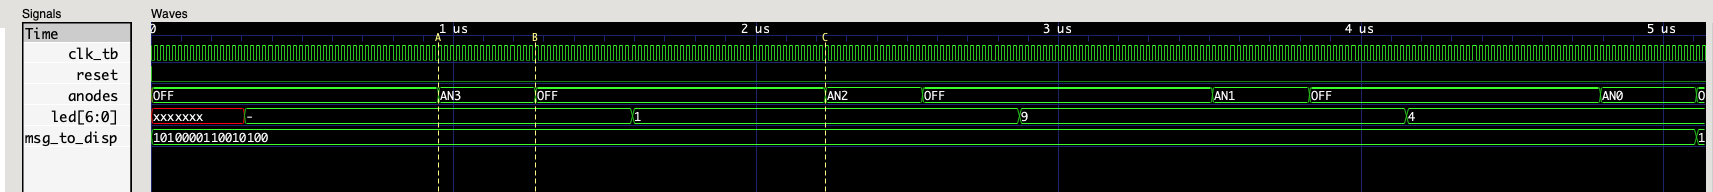
\includegraphics[width=\textwidth]{../images/led_driver_tb.png}
  \end{center}
  \caption{LedDriver4 testbench μεγέθυνση.}
  \label{fig:tb_led_driver}
\end{figure}

\end{document}
